	\section{MILP Models for global robustness}
	
	
	
	\subsection{Extending the classical encoding}
	
    To encode global robustness, \cite{vhagar} considers
	variable $x_j,\hat{x}_j$ and $x'_j,\hat{x}'_j$ for nodes of the image $I$ 
	and of its perturbation $I'$, 
	using the classical encoding (\ref{eq11}) \cite{MILP} 
	to compute $\hat{x}_i, \hat{x}'_i$ from $x_i, x'_i$
	for each $i$.
    Further:
    \begin{enumerate}
		\item For each input nodes $x_j,x'_j$ of $I,I'$, add constraints
        $|x_j-x'_j| \leq \varepsilon$ 
        ($L_\infty$-perturbation - see later for $L_1$).
		\item The optimization objective is to maximize $x_C - x_D +x'_D - x'_C$ 
		to compute $\beta^\varepsilon_{C,D}=\beta^\varepsilon_{D,C}$, 
		for $C \neq D$ two decision classes.
	\end{enumerate}

	We call this encoding $\mathcal{M}^{classical}$.
	It contains twice as many (binary) variables as for local robustness. 
	%As the worst-case complexity of solving an MILP model is exponential in the number of binary variables, it will be computationally intractable to compute $\beta^\varepsilon_{i,j}$ in this way, but for very small DNNs. 
	As explained in the previous section, the standard way to make the model more efficient is to rely on 
	linearly relaxing some of the binary variables into linear variables.

    The problem is that the LP relaxation of this classical encoding is extremely inaccurate, as variables $x_j,x'_j$ dependencies are due solely on the function definition through common ancestor variables in previous layers - as this is approximated with LP, most of the dependencies will be lost. On top of being an issue with partial MILP models, LP relaxation is also used during the Branch and Bound process internal to MILP solvers to provide bounds for each branch. So even when all variables are binary, the classical MILP encoding 
	of \cite{MILP}, while fully accurate, will likely not result into accurate bounds as well. Notice that this was already witnessed in \cite{ITNE}, and some additional constraints were added to make the classical model more accurate:
	the diff variables were defined, although to pass the ReLU the classical  
	MILP encoding was used, but with added specific constraints (Eq. (3) in 
	\cite{ITNE}). We will compare the different methods in Table \ref{table.classical}.

	

 


	\subsection{A novel "2v" model with {\em diff variables}}

	We now present our novel faithful "2v" model.
    First, we consider variables $x'_j,\hat{x}'_j, y_j, \hat{y}_j$, where $y_j, \hat{y}_j$ are the {\em diff variables}, with     $y_j = x_j - x'_j$ and $\hat{y}_j= \hat{x}_j - \hat{x}'_j$, as already proposed in \cite{lipshitz,ITNE}. 	Intuitively, the diff variables will be small as they will be carrying the difference between both the image $I$ and its perturbation $I'$.
    We will use the classical MILP encoding for $\hat{x}'_j$.

    However, unlike the Interleaving Twin-Network Encoding (ITNE) of \cite{lipshitz,ITNE} which relies on the classical MILP encoding (\ref{eq11}) \cite{MILP} to compute $\hat{y}_j$ from the difference between 
	$\ReLU(x'_j + y_j) = \ReLU(x_j) = \hat{x_j}$
	and $\hat{x}'_j$, we compute $\hat{y}_j$ directly, without resorting to the classical encoding. To do so, we study the function of 
    $\hat{y}_j$ given $y_j$ and $x'_j$, and encode it into a novel MILP model.
    A first important observation is that $I,I'$ being perfectly symmetrical,
    assuming that $\gamma_i$ is an upper bound of $y_i$, then $-\gamma_i$ is a lower bound for $y_i$.

	%	(This model has the same binary set, although the meaning of binary variable for $y_i$ is somehow different.)
	
	%	The exact constraints for $$ \begin{align*}
		%		&\hat{y}_i \geq -\hat{x}'_i \hspace*{1ex} \wedge \hspace*{1ex} \hat{y}_i \leq -\hat{x}'_i+a\beta_i  \hspace*{1ex}\wedge\hspace*{1ex} x_i'+y_i \leq a\beta_i \hspace*{1ex}\wedge\hspace*{1ex}  x_i'+y_i \geq (1-a)\alpha_i \\
		%		&\hat{y}_i \geq -\hat{x}'_i+(x_i'+y_i) \hspace*{1ex}\wedge\hspace*{1ex} \hat{y}_i \leq -\hat{x}'_i+(x_i'+y_i) +(a-1)\alpha_i \\
		%	\end{align*} 
	%	
	%	
	%	Moreover, we can add two more natural constraints: $x_i'+y_i \geq \alpha_i \hspace*{1ex}\wedge\hspace*{1ex}  x_i'+y_i \leq \beta_i.$
	
	We first display on Figure \ref{fig.2v} the function $f(x'_i,y_i)=\hat{y}_i$, granted that $y_i \in [- \gamma_i, \gamma_i]$. 
	When $x'_i \leq 0$ and $x_i = x'_i+y_i \leq 0$, then we have $\hat{y}_i = \ReLU(x_i) - \ReLU(x'_i) = 0-0=0$. For $x'_i \geq 0$ and $x_i = x'_i+y_i \geq 0$, we have $\hat{y}_i=
    \ReLU(x_i)-\ReLU(x'_i)=x_i - x'_i = y_i$. 
    Between these two linear planes, we have two more linear planes presenting intermediate cases, so 4 linear planes in total.
	
	\begin{figure}[t!]
		\centering
	\hspace*{-5ex}
	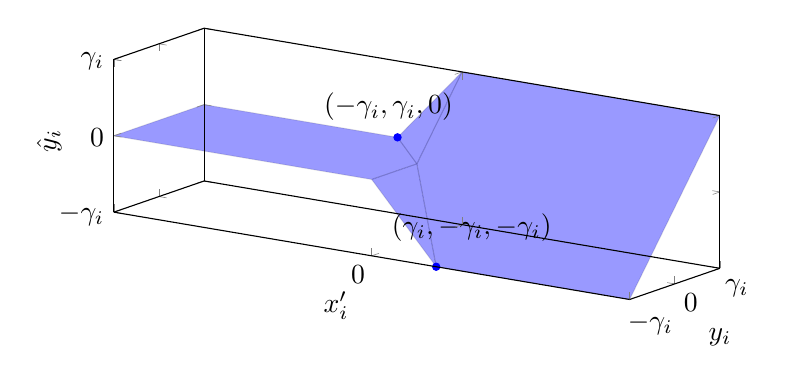
\begin{tikzpicture}[scale=0.65]
		\begin{axis}[	axis on top, xlabel = \(x'_i\),
			ylabel = {\(y_i\)}, zlabel = \(\hat{y}_i\),
			set layers=default,
			xmax = 4, xmin = -4,
			ymax = 1, ymin = -1,		
			zmax = 1, zmin = -1,
			unit vector ratio=1 1 1, scale=2.5,  ytick   = {-1,0,1},
			yticklabels = {$-\gamma_i$,$0$,$\gamma_i$}, xtick = {0},
			xticklabels = {$0$}, ztick   = {-1,0,1},
			zticklabels = {$-\gamma_i$,$0$,$\gamma_i$},
			view={35}{14},
			]
			\addplot3[ fill=blue,opacity=0.1, fill opacity=0.4] 
			coordinates {
				(0,0,0) (-1,1,0) (-4,1,0) (-4,-1,0) (0,-1,0) (0,0,0)
			};
			
			\addplot3[	fill=blue,opacity=0.1, fill opacity=0.4] 
			coordinates { (0,0,0) (0,1,1) (4, 1, 1) (4, -1, -1) (1,-1,-1) (0,0,0)
			};
			
			\addplot3[	fill=blue,opacity=0.1, fill opacity=0.4	] 
			coordinates { (0,0,0)  (-1,1,0) (0,1,1) (0,0,0)
			};
			
			\addplot3[	fill=blue,opacity=0.1, fill opacity=0.4	] 
			coordinates { (0,0,0)  (0,-1,0) (1,-1,-1) (0,0,0)
			};
			
			\addplot3[only marks, mark=*, mark size=2pt, blue] coordinates {(1,-1,-1)};
			\node[label={$(\gamma_i,-\gamma_i, -\gamma_i)$}] at (axis cs: 1.2, -0.5 ,-1) {};
			
			\addplot3[only marks, mark=*, mark size=2pt, blue] coordinates {(-1,1,0)};
			\node[label={$(-\gamma_i,\gamma_i, 0)$}] at (axis cs: -1, 0.8 ,0) {};			
		\end{axis}
	\end{tikzpicture}
	\caption{The function computing $\hat{y}_i=\ReLU(x_i)-\ReLU(x'_i)$ 
	depending on $y_i = x_i- x'_i$ and on $x'_i$.}
	\label{fig.2v}
\end{figure}
	

Recall first that we use the classical MILP encoding 
for $\hat{x}'_i=\ReLU(x'_i)$, using one binary variable $a'$. We reuse 
$a'$ (with its value already settled, see Proposition \ref{Prop1}) 
in the encoding of $\hat{y}_i = \ReLU(x_i)-\ReLU(x'_i)$:

\newpage

\begin{proposition}
    \label{Prop2}
Assuming that $y_i \in [-\gamma_i, \gamma_i]$,
and that $x'_i \in [\alpha_i,\beta_i]$,
we have that $\hat{y}_i = \ReLU(x_i=x'_i+y_i)-\ReLU(x'_i)$ is the solution of:
	\begin{align*}
		& \begin{aligned}
			y_i + x'_i &\leq a\beta_i        &
			y_i &+ x'_i \geq (1-a)\alpha_i \\
			x'_i       &\leq a'\beta_i       & 
			x'_i       &\geq (1-a')\alpha_i \\
			\hat{y}_i  &\leq a\gamma_i       &
			\hat{y}_i  &\geq -a'\gamma_i \\
			\hat{y}_i  &\leq y_i + (1-a)\gamma_i  &
			\hat{y}_i  &\geq y_i - (1-a')\gamma_i \\
			\hat{y}_i  &\leq -x'_i + a\beta_i &
			\hat{y}_i  &\geq -x'_i + (1-a')\alpha_i \\
			\hat{y}_i  &\leq y_i + x'_i + (1-a)(-\alpha_i) &
			\hat{y}_i  &\geq y_i + x'_i + a'(-\beta_i)
		\end{aligned}
	\end{align*} 
    where $a,a' \in \{0,1\}$ are binary variables, 
    and $a'$ is shared with the classical MILP
    encoding for $\hat{x}'_i=\ReLU(x'_i)$.
\end{proposition}

So to encode both $\hat{y}_i$ and $\hat{x}_i$, we need 2 binary variables altogether, similar to the classical encoding. The proof of Prop. \ref{Prop2} can be found in the supplementary materials.


The LP relaxation of this model contains important bounds, including 
    $\frac{y_i-\gamma_i}{2} \leq \hat{y}_i \leq \frac{y_i+\gamma_i}{2}$
    (see subsection The eficient "1v" model for a formal sketch), which is not the case of the classical model.
	

	\iffalse
\paragraph{A proof of Prop.~\ref{Prop2}}

We do a case analysis depending on the value of both binary variables. 
First, we know the constraints for $\hat{x_i}'=\ReLU(x_i')$ are exact (see 
Prop.~\ref{Prop1}). 

We have 2 binary variables and 4 cases in total. We only need to check that, in all 4 cases, $$\hat{y}_i = \ReLU(x'_i+y_i)-\ReLU(x'_i).$$

Case 1: if $a = 1$ and $a' = 1$, then $x'_i \geq 0 $ and $y_i+x'_i\geq 0$, then we need to show $\hat{y}_i = y_i$ based on  $\hat{x'_i} = x'_i$. This is true by the two inequalities in line 4.

Case 2: if $a = 1$ and $a' = 0$, then $x'_i \leq 0 $ and $y_i+x'_i\geq 0$, then we need to show $\hat{y}_i = y_i+x'_i$ based on  $\hat{x'_i} = 0$. This is true by the two inequalities in line 6.

Case 3: if $a = 0$ and $a' = 0$, then $x'_i \leq 0 $ and $y_i+x'_i\leq 0$, then we need to show $\hat{y}_i = 0$ based on  $\hat{x'_i} = 0$. This is true by the two inequalities in line 3.


Case 4: if $a = 0$ and $a' = 1$, then $x'_i \geq 0 $ and $y_i+x'_i\leq 0$, then we need to show $\hat{y}_i = -x'_i$ based on  $\hat{x'_i} = x'_i$. This is true by the two inequalities in line 5.

\fi

%\begin{proof}

%\end{proof}
	
	%	\begin{align*}
		%		& y_i+x'_i \leq a\beta_i \quad\wedge \quad y_i+x'_i\geq (1-a)\alpha_i\\	
		%		& x_i' \leq a'\beta_i \quad\wedge \quad x_i'\geq (1-a')\alpha_i\\
		%		&\hat{y}_i \leq a\gamma_i \quad\wedge \quad	\hat{y}_i \geq -a'\gamma_i \\
		%		&	\hat{y}_i \leq y_i+(1-a)\gamma_i \quad\wedge \quad	\hat{y}_i \geq y_i - (1-a')\gamma_i \\
		%		&	\hat{y}_i \leq -x'_i+a\beta_i \quad\wedge \quad	\hat{y}_i \geq -x'_i+(1-a')\alpha_i \\
		%		&	\hat{y}_i \leq y_i+x'_i+(1-a)(-\alpha_i)\quad\wedge \quad	\hat{y}_i \geq y_i+x'_i+a'(-\beta_i) \\
		%	\end{align*} 
	
	

	%	The relaxation of this model is similar: let $a$s and $a'$s be continuous variables instead of binary/integer variables. Unlike the first model in this section, relaxing a few nodes does not lose too much accuracy.
	
    
    
    


    \subsection{A decoupled "3v" model}

	Besides doing LP relaxation on some of the binary variables, we propose a 
    variant of the "2v" model: the binary variables $a'$ appearing in 
    Prop. \ref{Prop2} can be decoupled from the binary variable appearing in the classical encoding of $x'_i = \ReLU(x'_i)$. While this means having 3 binary variables per unstable ReLU (which warrants the name "3v" model), the fact that these variables are decoupled removes a lot of constraints in the MILP encoding, and actually helps the solver. The decoupling also means that the "3v" model is not as accurate as the "2v" model.


	\subsection{The efficient "1v" model}

		\begin{figure}[t!]
		\centering
	\hspace*{10ex}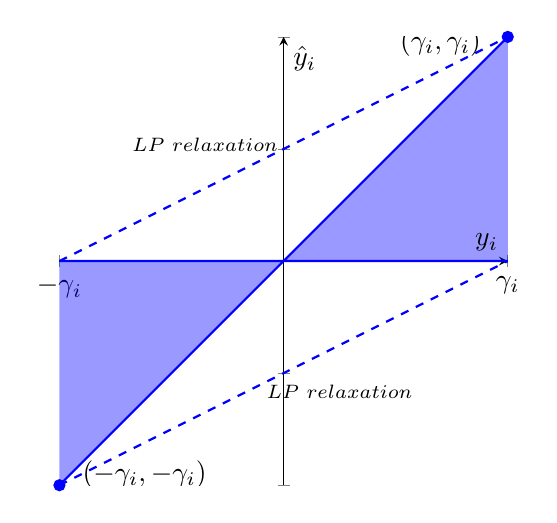
\begin{tikzpicture}
		\begin{axis}[
			xlabel={$y_i$},
			ylabel={$\hat{y}_i$},
			xmin=-2, xmax=2,
			ymin=-2, ymax=2,
			axis lines=center,
			samples=100, 
			unit vector ratio=1 1 1, scale=1, xtick   = {-2,2},
			xticklabels = {$-\gamma_i$,$\gamma_i$},
			yticklabels = {},
			]
			\addplot[blue, thick, fill=blue, fill opacity=0.4] {x} \closedcycle; 
			\addplot[blue, thick] {0}; 
			
			\addplot[only marks, mark=*, mark size=2pt, blue] coordinates {(-2,-2)};
			\node[label={above:$(-\gamma_i,-\gamma_i)$}] at (axis cs: -1.24, -2.2) {};
			
			\addplot[only marks, mark=*, mark size=2pt, blue] coordinates {(2,2)};
			\node[label={above:$(\gamma_i,\gamma_i)$}] at (axis cs: 1.4, 1.65) {};
		\addplot[dashed, thick, blue] coordinates {(-2,-2) (2,0)};
			\addplot[dashed, thick, blue] coordinates {(-2,0) (2,2)};
			\node[label={above:\scriptsize $LP\ relaxation$}] at (axis cs: -0.7, 0.8) {};
			\node[label={above:\scriptsize $LP\ relaxation$}] at (axis cs: 0.5, -1.4) {};
		\end{axis}
	\end{tikzpicture}
\caption{The possible values of $\hat{y}_i=\ReLU(x_i)-\ReLU(x'_i)$ depending on $y_i = x_i-x'_i$ for the "1v" model.}
	\label{fig.1v}
\end{figure}



	To simplify further and limit the number of (binary) variables, 
    we introduce an efficient "1v" model which only uses the diff variables $y_i,\hat{y}_i$. Again, we study the range of values $\hat{y}_i$ can take according to the value of $y_i$, as depicted in Fig.~\ref{fig.1v}. This is a projection of Fig.~\ref{fig.2v} onto $y_i,\hat{y}_i$.
    
\newpage

    \begin{proposition}
    \label{prop3}
    Given $y_i \in [-\gamma_i,\gamma_i]$, 
    $\hat{y}_i$ is a solution of the following MILP program :\begin{align*}
		\hat{y}_i &\leq a \gamma_i               &\quad \hat{y}_i &\geq y_i - a \gamma_i \\
		\hat{y}_i &\geq (a-1) \gamma_i           &\quad \hat{y}_i &\leq y_i + (1-a) \gamma_i
	\end{align*} where $a \in \{0,1\}$ is a binary variable.
	\end{proposition}

    We can easily check that the LP relaxation of this MILP program,
	depicted in broken lines on Fig.~\ref{fig.1v}, is exactly: 
    \begin{equation}
		\label{eq.lpr}
	  \frac{y_i-\gamma_i}{2} \leq \hat{y}_i \leq \frac{y_i+\gamma_i}{2}
	\end{equation}

	As the "1v" model is a projection of the "2v" and also of the "3v" models, 
	the LP relaxations of the "2v" and the "3v" models contain (\ref{eq.lpr}).
	Notice that (\ref{eq.lpr}) corresponds to Eq. (3) in \cite{ITNE}, 
	which is added explicitly to the classical model in their ITNE model.
	
    
	
	

	\iffalse
	Based on above constraints, we can sketch this simplified model:
	\begin{enumerate}
		\item For each input node, each output node, and each pre-activation and post-activation node in the hidden layers,  set one variable $y_i$. 
		\item Set constraints for input nodes.
		\item Set linear constraints . In this case, since the meaning of $y_i$ is $x_i-x'_i$, this constraints will not use the bias.
		\item Between pre- and post- activation nodes, set the MILP constraint described above.
	\end{enumerate}
	
	The key point is that, although this model sets 3 variables (and their binary variables) for each node in the network, only $y_i$  contributes to the final results, and we can ignore $x_i,x_i'$ (and their binary variables) during the optimization.
	
	As a result, we can relax the binary variables used to $\hat{x}_i = \ReLU(x_i)$ and $\hat{x}'_i = \ReLU(x'_i)$.
	\fi

	%The "1v" model contains the same number of (binary) variables as the MILP model for local robustness, but it is not as accurate as the "3v" or "2v" models. 
    
	%	However, in practice, with a reasonable timeout, this simplified model can usually obtain a better bound.
	%	


    